\documentclass{article}
\usepackage[utf8]{inputenc}
\usepackage[letterpaper, portrait, margin=1in]{geometry}
\usepackage{multicol}
\usepackage{amsmath}
\usepackage{amssymb}
\usepackage{enumerate}
\setlength\parindent{0pt}
\usepackage{enumerate}
\usepackage{graphicx}
\graphicspath{ {./images/} }
\usepackage{fancyhdr}
\usepackage{tcolorbox}
\usepackage{mathtools}
\newcommand{\sheader}[1]{\underline{#1:}}
\newcommand{\ftrans}{\xleftrightarrow[]{f}}
\newcommand{\ejw}{{e^\jomega}}
\newcommand{\curly}[1]{\left\{#1\right\}}
\usepackage{tabularx}

\newcommand{\header}[1]{\begin{large}\noindent #1\end{large}\\\rule{\textwidth}{0.5pt}}
\newcommand{\gap}{\medskip\\}
\newcommand{\centertext}[1]{\begin{center}#1\end{center}}
\newcommand{\bfrac}[2]{\left(\frac{#1}{#2}\right)}
\newcommand{\formula}[3]{\begin{center} \begin{tcolorbox}[title = #2] $$#3$$\end{tcolorbox}\end{center}}
\newcommand{\where}{\hspace{0.5cm} \textrm{where} \hspace{0.5cm}}
\newcommand{\hgap}{\hspace{0.5cm}}
\newcommand{\pfrac}[2]{\frac{\partial #1}{\partial #2}}
\newcommand{\jomega}{{j\omega}}
\newcommand{\domega}{d\omega}
\usepackage[scr]{rsfso}

\newcommand{\Laplace}{\mathscr{L}}
\newcommand{\Fourier}{\mathcal{F}}
\newcommand{\Laplacearrow}{\xleftrightarrow{\Laplace}}
\newcommand{\zarrow}{\xleftrightarrow{\mathcal{Z}}}

\newcommand{\doubleformula}[4]{\begin{center} \begin{tcolorbox}[title = #2] $$#3$$\\$$#4$$\end{tcolorbox}\end{center}}

\newcommand{\tripleformula}[5]{\begin{center} \begin{tcolorbox}[title = #2] $$#3$$\\$$#4$$\\$$#5$$\end{tcolorbox}\end{center}}

\title{ELEC 221 Notes}
\author{reesecritchlow }
\date{September 2022}

\begin{document}

\begin{center}
    \Large ELEC 221 Notes\\
    \normalsize Reese Critchlow
\end{center}

\header{Notation}

\begin{align*}
    \textrm{Continuous Signals} && \textrm{Discrete Signals}\\
    x(t) && x(n)\\
    \textrm{Continuous-Time Systems} && \textrm{Discrete-Time Systems}\\
    x(t) \to y(t) && x[n] \to y[n]
\end{align*}
The arrow for systems means that for a given signal, say $x(t)$ when in putted into a system ($\to$) yields an output signal $y(t)$.
\\\gap
An equals sign ($=$) simply indicates equality between two signals.
\\\gap
\header{System Properties}
\begin{enumerate}
    \item \textbf{Memory}\\
    A system is \underline{memoryless} if the output at each time depends only on the input at the same time.\\
    Examples:
    \begin{align*}
        \textrm{Example: Voltage Through a Resistor} && V(t) = RI(t)\\
        \textrm {Counter Example: Voltage through a Capacitor} && V(t) = \frac{1}{C}\int_{-\infty}^tI(\tau)d\tau \\
        \textrm{Counter Example: A Delay System} && y[n] = x[n-1]
    \end{align*}
    Generally, a system where the function has some sort of time depenence which is not in the instantaneous current time period has a memory.
    
    \item \textbf{Invertibility}\\
    A system is \underline{invertible} if distinct inputs lead to distinct outputs.\\
    An example of a noninvertible system is $y(t) = x^2(t)$, because the square destroys a negative sign that may have existed in the input signal.
    
    \item \textbf{Causality}\\
    A system is \underline{causal} if the output at \textit{any time} depends only on the input at the present time or in the past. A comparison between causal systems and systems with memories may be able to be drawn, but they are not the same.
    \begin{multicols}{2}
        \underline{Causal Systems}
        \begin{itemize}
            \item Dependent events can only be in the present or in the past.
        \end{itemize}
        \vfill\null\columnbreak
        \underline{Memory-Bearing Systems}
        \begin{itemize}
            \item Dependent events can be in the present or in the future.
        \end{itemize}
        \vfill\null
    \end{multicols}
    A capacitor is causal, but a moving average, or time reversal is not.
    \item \textbf{Stability}\\
    A system is \underline{stable} if small changes in input do not cause the output to diverge.\\
    A stable system can also be described as one where bounded inputs lead to bounded outputs; essentially that the system never reaches an unbounded value.\\
    A system is also stable if \underline{the impulse response is absolutley integrable}.
    \item \textbf{Time Invariance}\\
    A system is \underline{time invariant} if time shifts in the input lead to identical time shifts in the output.\\
    \gap
    \underline{Proving Time Invariance}: Shift the input signal by a time period $a$, and pass it through the system. Shift the un-shifted output signal of the system by the same time period $a$. If they are the same signal, the system is time invariant.
    \item \textbf{Linearity}
    A \underline{linear} system has the following properties:
    
    \begin{center}
        \begin{multicols}{2}
            \underline{Additivity}
            \[
                x_1(t) + x_2(t) \to y_1(t) + y_2(t)
            \]
            \vfill\null\columnbreak
            \underline{Homogeneity}
            \[
                ax_1(t) \to ay_1(t)
            \]
            \vfill\null
        \end{multicols}
    \end{center}
    
    These two properties can also be combined:
    \[
        ax_1(t) + bx_2(t) \to ay_1(t) + by_2(t)
    \]
    
\end{enumerate}

\header{Harmonics}
A signal that has \textbf{only odd harmonics} requires that:
\[
    f\left(t+\frac{T}{2}\right) = -f(t)
\]
Whereas a signal that has \textbf{only even harmonics} requires that:
\[
    f\left(t + \frac{T}{2}\right) = f(t)
\]

\header{Impulse Response}

The \textbf{Impulse Response} of a system is the signal a system produces after a
unit impulse signal is passed through it. The unit impulse response is denoted by:
\begin{align*}
     h(n) && h[n].
\end{align*}
The impulse response is generally used to determine the ouput of a system 
by means of the convolution.
\gap
\header{Convolution}

The \textbf{Convolution} operation multiplies the entries of one signal by another in
a systematic fashion. It is defined by:
\begin{align*}
    x(t) \ast h(t) = \int_{-\infty}^\infty x(\tau) h(t- \tau) {d}\tau && x[n] \ast h[n] = \sum_{k=-\infty}^\infty x[k]h[n-k]    
\end{align*}
In this context, the convolution operator is being used to determine the output of a
signal through a system, given the system's impulse response.
\gap
\underline{Properties of the Convolution:} The convolution is:
\begin{itemize}
    \item Associative: $x \ast (y \ast z) = (x \ast y) \ast z$
    \item Commutative: $x \ast y = y \ast x$
    \item Distributive: $x \ast (y + z) = x \ast y + x \ast z$
\end{itemize}

\pagebreak

\header{Fourier Series (Continuous Time)}

Given a correct periodic signal, one can describe it as a sum of complex exponentials,
called a \textbf{Fourier Series}. 
\gap
Signals that can be expressed as a fourier series must obey the \underline{Dirichlet Conditions}:
\gap
If over one period, a signal $x(t)$:
\begin{enumerate}
    \item Is single-valued
    \item Is absolutley integrable
    \item Has a finite number of maxima and minima
    \item Has a finite number of discontinuities
\end{enumerate}
The Dirichlet conditions are sufficient but \underline{not necessary}, however. This
being said, they can tell us that the Fourier series \underline{converges} to:
\begin{itemize}
    \item $x(t)$ where it is continuous
    \item half the value of the jump if it is discontinuous.
\end{itemize}


The Fourier Series has two parts to it:
\begin{multicols}{2}
    \centertext{\underline{Fourier Synthesis Equation}}
    \[
        x(t) = \sum_{k = -\infty}^\infty c_k e^{jk\omega t}    
    \]
    \centertext{where $\omega$ is the fundamental frequency of the function.}
    \vfill\null\columnbreak
    \centertext{\underline{Fourier Analysis Equation}}
    \[
        c_k = \frac{1}{T}\int_T e^{-jk\omega t}x(t){d}t    
    \]
    \centertext{where $T$ is the period of the function.}
    \vfill\null
\end{multicols}

\underline{Gibbs Phenomena:} If a function represented by a Fourier series has discontinuities,
there will be ``imperfections'' or ``ringings'' in the Fourier series. This is known
as the Gibbs Phenomena, where it is known that there will be ``spikes'' of about $9\%$
the height of the discontinuity around the bounds of the discontinuity itself.
\gap
\header{Operations on Fourier Series}

\underline{Summation of Signals}
\smallskip\\
Given two signals with the same period:
\begin{align*}
    x_1(t) = \sum_{k = -\infty}^\infty c_{k(1)}e^{jk\omega t} && x_2(t) = \sum_{k = -\infty}^\infty c_{k(2)}e^{jk\omega t}
\end{align*}
Then we can find their sum as:
\begin{align*}
    y(t) = Ax_1(t) + Bx_2(t) = \sum_{k = -\infty}^\infty c_k e^{jk\omega t} && c_k = Ac_{k(1)} + Bc_{k(2)}
\end{align*}
\underline{Time Shifting}
\smallskip\\
Given a signal, its timeshift, $x(t) \to x(t - t_0)$ can be obtained by:
\begin{align*}
    x(t - t_0) = \sum_{k = -\infty}^\infty c'_k e^{jk\omega t} && c'_k = e^{-jk\omega t_0}\cdot c_k
\end{align*}
\underline{Convolution of Signals}
Given two signals with the same fundamental frequency*:
\begin{align*}
    x_1(t) = \sum_{k = -\infty}^\infty c_{k(1)}e^{jk\omega t} && x_2(t) = \sum_{k = -\infty}^\infty c_{k(2)}e^{jk\omega t}
\end{align*}
Then the convolution of the signals takes the form of:
\begin{align*}
    y(t) = x_1(t) \ast x_2(t) = \sum_{k = -\infty}^\infty c_k' e^{jk\omega t} && c'_k = \sum_{l = -\infty}^\infty a_l b_{k - l}
\end{align*}
\gap
\header{Signal Power and Energy}

We can define the power and energy of a periodic function over a single period. 
\begin{multicols}{2}
    \centertext{\underline{Energy of a Signal}}
    \[
        E = \int_T \left|x(t)\right|^2 dt    
    \]
    \vfill\null\columnbreak
    \centertext{\underline{Power of a Signal}}
    \[
        P = \frac{1}{T}\int_T \left|x(t)\right|^2 dt    
    \]
    \vfill\null
\end{multicols}

Power and energy can also be used to show \underline{Parseval's Relation}.

\[
    \frac{1}{T}\int_T\left|x(t)\right|^2 dt = \sum_{k = -\infty}^\infty |c_k|^2    
\]

\header{Discrete Time Fourier Series}
\underline{Precursor -- Differences between DT and CT periodic signals}: There are 
two main differences between DT and CT periodic signals. 
\begin{enumerate}
    \item Frequency does not increase infinitley with $\omega$.
    \smallskip\\
    For some $x[n]$ with period T:
    \begin{align*}
        x[n] &= e^{\frac{2\pi n}{T}j}\\
        &= e^{\frac{2\pi (n + N)}{T}j}\\
        &= e^{\frac{2\pi n}{T}j}e^{\frac{2\pi N}{T}j}\\
        & \textrm{But if } N > T,\\
        &= e^{\frac{2\pi n}{T}j}e^{\frac{2\pi (T\alpha + N')}{T}j}\\
        &= e^{\frac{2\pi n}{T}j}e^{\frac{2\pi (N')}{T}j}e^{{2\pi \alpha}j}\\
        &= e^{\frac{2\pi n}{T}j}e^{{2\pi (N')}}
    \end{align*}
    It is important to note that this same result does not hold in CT because the
    resolution of $\alpha$ is not restricted to $\mathbb{Z}$.
    \item $\frac{\omega}{2\pi}$ must be rational for the signal to be periodic.
    \gap
    \underline{Note:} If $\frac{\omega}{2\pi}$ is a fraction, the numerator is the period.
\end{enumerate}
Now, we can define the Fourier synthesis and analysis equations for discrete time.
\begin{multicols}{2}
    \centertext{\underline{Fourier Synthesis Equation}}
    \[
        x[n] = \sum_{k = 0}^{N - 1}c_k e^{jk \frac{2\pi n}{N}}   
    \]
    \centertext{where $N$ is the period or number of samples of the function.}
    \vfill\null\columnbreak
    \centertext{\underline{Fourier Analysis Equation}}
    \[
        c_k = \frac{1}{N}\sum_{n = 0}^{N - 1}x[n]e^{-jk \frac{2\pi n}{N}}   
    \]
    \centertext{where $N$ is the period or number of samples of the function.}
    \vfill\null
\end{multicols}

\header{The Frequency Response}

The \textbf{Frequency Response} or the \textbf{System Response} of a system, denoted
by $H(j\omega)$ describes how frequencies are attenuated, amplified, and phase shifted
in a system. 
\smallskip\\
It is computed by:
\begin{align*}
    H(j\omega) = \int_{-\infty}^\infty e^{j\omega \tau}h(\tau){d}\tau 
\end{align*}
\underline{Question:} Are there frequency responses in DT?
\gap
\underline{Using the Frequency Response:} To use the frequency response, to compute
how a system changes a signal, there are three steps.
\begin{enumerate}
    \item Compute the frequency response (if it isn't already given).
    \item Compute the Fourier coefficients of the signal.
    \item Apply the frequency response to each of the Fourier coefficents to obtain
    the output signal.
\end{enumerate}
This can be generalized to:
\begin{align*}
    x(t) \to y(t) = \sum_{k = -\infty}^\infty c_k H(jk \omega)e^{jk\omega t} &&
    x[n] \to y[n] = \sum_{k = 0}^{N - 1}c_k H(e^{jk\omega})e^{jk\omega n}
\end{align*}

\header{Filters}
We can characterize filters by their frequency responses, $H$.
\gap
\underline{Filters in Discrete Time:} It is important to note that a filter in DT
is mirrored across zero. Frequencies increase up until $\omega = \pi$ and then
subsequently decrease.
\gap
\underline{Categories of Filters:} Filters can be broken up into two main categories:
\begin{enumerate}
    \item Infinite Impulse Response (IIR)\\
    Infinite impulse response filters are those whose impulse response \underline{does not}
    become zero over a finite amount of time.
    \item Finite Impulse Response (FIR)\\
    Finite impulse response filters are thos whose impulse response \underline{does} 
    become zero over a finite amount of time.
\end{enumerate}

\pagebreak

\header{The Fourier Transform}
The \textbf{Fourier Transform}, not to be confused with the \textit{Fourier series}
employs the principles of the \textit{Fourier series} to \underline{aperiodic signals}.
Thus, the equations governing it are:

\begin{multicols}{2}
    \centertext{\underline{Inverse Fourier Transform}}
    \[
        x(t) = \frac{1}{2\pi}\int_{-\infty}^\infty X(j\omega)e^{j\omega t}{d}\omega
    \]
    \vfill\null\columnbreak
    \centertext{\underline{Fourier Transform (Fourier Spectrum)}}
    \[
        X(\jomega) = \int_{-\infty}^\infty x(t)e^{-\jomega t}{d}t  
    \]
    \vfill\null
\end{multicols}
A more physical intuition of the Fourier transform is that it takes
a signal and decomposes it into a spectrum of its frequencies. This
is called the \underline{Fourier Spectrum}.
\gap
\underline{Fourier Transform and Impulse Response:} The Fourier
transform can be used to obtain the frequency response from the impulse response
and vice versa. This forwards direction of this was already known however.

\begin{multicols}{2}
    \centertext{\underline{Continuous Time}}
    \begin{align*}
        h[n] &= \frac{1}{2\pi}\int_{2\pi}H(e^\jomega)e^{\jomega n} \domega\\
        H(\jomega) &= \int_{-\infty}^\infty e^{-\jomega \tau}h(\tau)d\tau
    \end{align*}
    \vfill\null\columnbreak
    \centertext{\underline{Discrete Time}}
    \begin{align*}
        h(t) &= \frac{1}{2\pi}\int_{-\infty}^\infty e^{j\omega t}H(\jomega)\domega \\ 
        H(e^{\jomega}) &= \sum_{n = -\infty}^\infty e^{-\jomega n }h[n]
    \end{align*}
    \vfill\null
\end{multicols}

\pagebreak

\section*{Midterm 2}

\header{Properties of Fourier Transforms}

\sheader{Multiplication Property} We can shift the frequency spectrum of a signal by using the \underline{multiplication property}.
This comes in the form:
\begin{align*}
    x(t) \cdot e^{j\omega_c t} \xleftrightarrow[]{f}  X(j(\omega - \omega_0))
\end{align*}

\sheader{Differentiation} Differentiation also is made easy under 
Fourier transforms.

\begin{align*}
    \frac{dx(t)}{dt} \ftrans \jomega X(jw)
\end{align*}

\sheader{Integration}

\begin{align*}
    \int_{-\infty}^t x(\tau) d\tau \ftrans \frac{1}{\jomega}X(\jomega) + \pi X(0)\delta(\omega)
\end{align*}

We can also chain all of these together with successive multiplications
in the frequency domain.
\gap
\sheader{Differential Equations under Fourier Transforms} One can obtain
the transfer function of a differential equation under a fourier transform.
Given a differential equation of the form:
\begin{align*}
    \sum_{k = 0}^N \alpha_k \frac{d^ky(t)}{dt^k} = \sum_{k = 0}^M \beta_k \frac{d^k x(t)}{dt^k}
\end{align*}
We can obtain its transfer function:
\begin{align*}
    H(j\omega) = \frac{Y(\jomega)}{X(\jomega)} = \frac{\sum_{k = 0}^M \beta_k (\jomega)^k}{\sum_{k = 0}^N\alpha_k(\jomega)^k}
\end{align*}
This formula is kind of confusing. It's important to just note it as:
\begin{align*}
    H(\jomega) = \frac{\sum x\textrm{ coeffs}\cdot (\jomega)^k}{\sum y \textrm{ coeffs} \cdot (\jomega)^k}
\end{align*}
\sheader{Difference Equations under Fourier Transforms} 
We can also apply the same formulae to difference equations:
\begin{align*}
    \sum_{k = 0}^N \alpha_k y[n - k] = \sum_{k = 0}^M \beta_k x[n - k]
\end{align*}
Thus, resulting in a similar formula:
\begin{align*}
    H(e^\jomega) = \frac{Y(\jomega)}{X(\jomega)} = \frac{\sum_{k = 0}^M \beta_k e^{-jk\omega}}{\sum_{k = 0}^M \alpha_k e^{-jk\omega}} = \frac{\sum x \textrm{ coeffs} \cdot e^{-jk\omega}}{\sum y \textrm{ coeffs} \cdot e^{-jk\omega}}
\end{align*}

\pagebreak

\header{The Discrete Time Fourier Transform}

The \underline{Discrete Time Fourier Transform} is used for transforming
\textbf{discrete, aperiodic signals}. It is as follows:
\begin{multicols}{2}
    \centertext{\underline{Inverse DTFT (Synthesis)}}
    \begin{align*}
        x[n] = \frac{1}{2\pi}\int_{2\pi}X(e^\jomega)e^{\jomega n}d\omega
    \end{align*}
    \vfill\null\columnbreak
    \centertext{\underline{DTFT (Analysis)}}
    \begin{align*}
        X(e^\jomega) = \sum_{n = -\infty}^\infty x[n] e^{-j\omega n}
    \end{align*}
    \vfill\null
    
\end{multicols}

We also require \underline{convergence criteria} in the DTFT. It is as follows:
\begin{align*}
    \sum_{n=-\infty}^\infty | x[n] | < \infty && \sum_{n = -\infty}^\infty |x[n]|^2 < \infty
\end{align*}
Only \underline{one} of these criteria must be satisfied.
\gap
There exist the same properites for the CT Fourier transform, however, some more
properties aries in the DTFT:
\gap
\sheader{Conjugation} 

\begin{align*}
    \textrm{Even}(x[n]) \ftrans \textrm{Re}(X(\ejw)) && \textrm{Odd}(x[n]) \ftrans j\cdot \textrm{Im}(X(\ejw))
\end{align*}

\sheader{Periodicity}
\begin{align*}
    X(e^{j(\omega + 2\pi)} = X(\ejw))
\end{align*}

\sheader{Differentiation in Frequency} (Warning: this is \underline{very} different.)
\begin{align*}
    n \cdot x[n] \ftrans j \frac{d X(\ejw)}{d\omega}
\end{align*}

\sheader{Differencing}
\begin{align*}
    x[n] - x[n - 1] \ftrans (1 - e^{-\jomega} )X(\ejw)
\end{align*}

\sheader{Accumulating}
\begin{align*}
    \sum_{m = -\infty}^n x[m] \ftrans  \frac{1}{1 - e^{-\jomega}}X(\ejw) + \pi X(e^{j0})\sum_{k = -\infty}^\infty \delta(w - 2\pi k)
\end{align*}

\sheader{Parseval's Theorem} We can also define Parseval's theorem in the DTFT.
\begin{align*}
    \sum_{n = -\infty}^\infty |x[n]|^2 = \frac{1}{2\pi} |X(\ejw)|^2 d\omega
\end{align*}

\header{The Fast Fourier Transform}

It's cool. It has $N\log_2{N}$ time complexity.

\pagebreak

\header{Frequency Responses of LTI Systems}

We can look at the frequency responses of LTI systems with a slightly different prespective.
\gap
Since a transfer function, $H(\jomega)$ or $H(\ejw)$ has both a magnitude and a phase,
we can write a transfer function, or any frequency spectrum as:
\begin{align*}
    H(\jomega) = |H(\jomega)| e^{\angle H(\jomega)}
\end{align*}

Hence, we can write input and ouptut signals as follows:
\begin{align*}
    |Y(\jomega)| &= |H(\jomega)||X(\jomega)| \\
    \angle Y(\jomega) &= \angle H(\jomega) + \angle X(\jomega)
\end{align*}

\sheader{Group Delay} We can also define how much a system delays its input signal
through the \underline{group delay}. 
\begin{align*}
    \tau(\omega) = -\frac{d}{d\omega} \left(\angle H(\jomega)\right)
\end{align*}

\header{Step Response}

Under an ideal filter, a step function attains some sort of ``ringing'' in the
graph. Thus, we find it important to define the \underline{step response}
for systems.
\gap
Computing the step response is as follows:
\begin{align*}
    s(t) = \int_{-\infty}^t h(\tau) d\tau
\end{align*}

\header{Bode Plots}

Often, we find ourselves in situations where plotting phase and magnitudes of transfer
functions is difficult because of multiplication/division. Thus, we can use a 
\underline{Bode Plot}. The process for obtaining a Bode Plot is as follows:

\begin{multicols}{2}
    \centertext{\underline{Magnitude}}
    \begin{enumerate}
        \item Take $-20\log_{10}|H(\jomega)|$
        \item Identify the point(s), $\tau_n$ for which the function has an 
        ``inflection point''.
        \item Take $\omega \gg \tau_n$ and $\omega \ll \tau_n$, and plot 
        the two behaviours.
    \end{enumerate}
    \vfill\null\columnbreak
    \centertext{\underline{Phase}}
    \begin{enumerate}
        \item Plot against $\log_{10}\omega$.
    \end{enumerate}
\end{multicols}

\pagebreak

\header{Sampling Theory}
Given a signal $x(t)$, we can define an ``impulse train'' $p(t)$, which is a train
of impulses that ``sample'' our signal at a given interval $T$. We can also
define our \underline{sampling frequency} to be:
\begin{align*}
    \omega_s = \frac{2\pi}{T}.
\end{align*}

Hence, we can define our \underline{sampled signal} $x_p(t) = x(t) \cdot p(t)$.
\begin{align*}
    x_p(t) = \sum_{n = - \infty}^\infty x(nT) \cdot \delta(t - nT).
\end{align*} 

Given a sampled signal, it is natural to investigate the frequency spectrum of 
$x(t)$, $p(t)$, and $x_p(t)$. Hence, we can derive the Fourier transforms for each:
\begin{multicols}{3}
    \centertext{\underline{$X(\jomega)$}}
    \begin{align*}
        X(\jomega) = X(\jomega)
    \end{align*}
    \vfill\null\columnbreak
    \centertext{\underline{$P(\jomega)$}}
    \begin{align*}
        P(\jomega) = \frac{2\pi}{T}\sum_{k = \infty}^\infty \delta(\omega - k\omega_s)
    \end{align*}
    \vfill\null\columnbreak
    \centertext{\underline{$X_p(\jomega)$}}
    \begin{align*}
        X_p(\jomega) = \frac{1}{T} \sum_{k = -\infty}^\infty X(j(\omega - k\omega_s))
    \end{align*}
    \vfill\null
\end{multicols}

It's also very important to get a grasp on the graphs that result from these functions:
\\
\begin{center}
    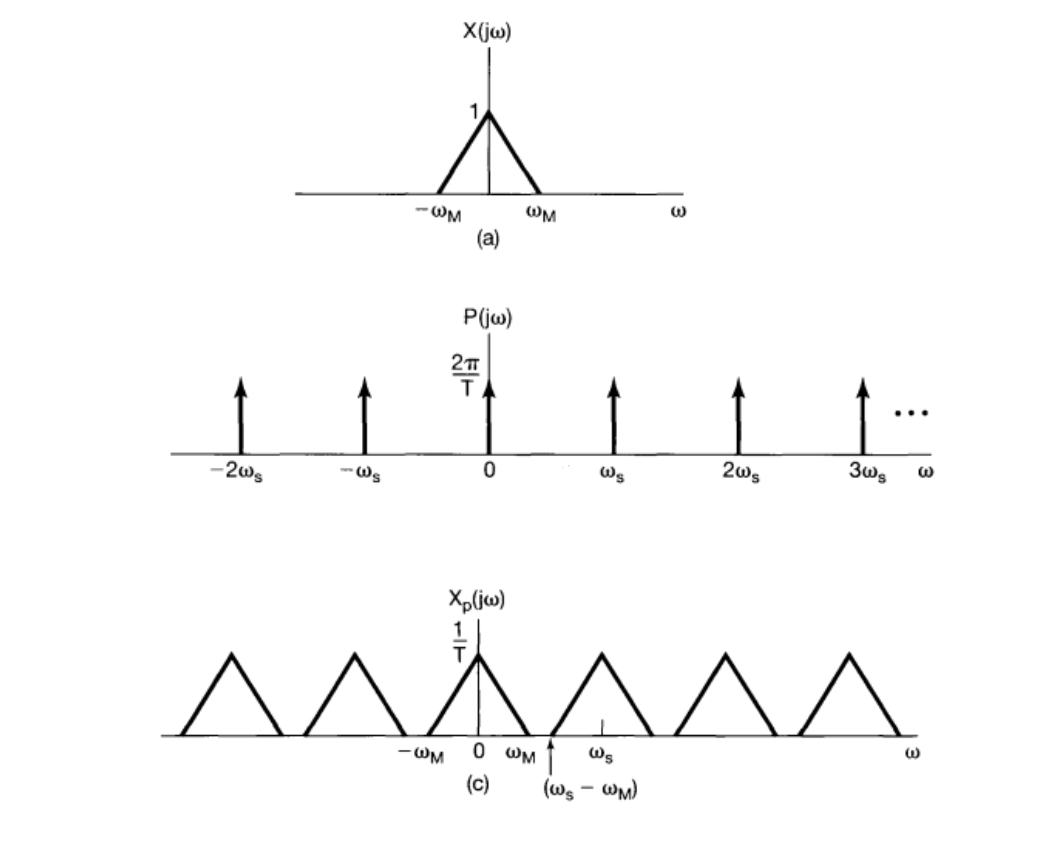
\includegraphics[scale=0.45]{sampling-graphs.png}    
\end{center}
Note that for the graph of $X_p(j\omega)$ has the $\omega_s - \omega_m$, which will
be important later. $\omega_m$ is defined as the maximum frequency contained in the
input signal.
\gap
Hence, the question may be posed: How can retrieve the original signal from the
sampled signal? The answer to this question is the \textbf{Sampling Theorem}:
\gap
\sheader{Sampling Theorem (condensed)}
Any signal can be reconstructed if the sampling frequency is \textit{strictly} larger than twice
the maximum frequency in the sampled signal. In math, this looks like:
\begin{align*}
    \omega_s > 2\omega_m
\end{align*} 
Hence, we can also define:
\begin{itemize}
    \item \sheader{Nyquist Rate} $\omega_s = 2\omega_M$
    \item \sheader{Nyquist Frequency} $\omega_M = \omega_s / 2$
\end{itemize}

\pagebreak

\header{Interpolation}
Often, we cannot always fully reconstruct our signal from the sampled signal, due
to a sampling rate that is too low. Hence, there are some methods in which 
we can \textit{interpolate} the sampled signal to attempt to reconstruct the 
original signal. Some of these methods include, but are not limited to:
\begin{itemize}
    \item \sheader{Zero Order Hold} Assume each point maintains the same value
    until the next sample is available.
    \item \sheader{Band Limited Interpolation} Apply a lowpass filter to the 
    system, with cutoff $\omega_c$ and gain $T$.
    \begin{align*}
        x_r(t) = \sum_{n = \infty}^\infty x(nT)\frac{\omega_c T \sin(\omega_c(t - nT))}{\pi \omega_c(t - nT)}
    \end{align*}
\end{itemize}

\header{Aliasing}

An important phenomena arises when you don't sample at a high enough rate: \textbf{aliasing}.
\gap
Essentially, the frequencies in $X_p(\jomega)$ begin to overlap, and the frequency
spectrum of the original spectrum becomes distorted.
\gap
\header{Conversions Between DT and CT}

Many common computing practices see the conversion of a signal from CT to DT and then
back to CT in order to employ computational methods of signal processing. For such
a process, we define a standard process for such signal processing.

\begin{enumerate}
    \item Original signal $x_c(t)$ is sampled by an impulse train $p(t)$ to form
    the sampled signal $x_p(t)$.
    \item Sampled signal is converted to a discrete time signal $x_d[n]$.
    \item Discrete signal is processed through $H_d(\ejw)$.
    \item Processed, discrete signal is transformed back into a CT signal.
    \item CT signal is low-passed to recover the original signal.
\end{enumerate}

Hence, when converting to a DT signal, we find ourselves with a new frequency 
defining our Fourier spectrum, $\Omega$.
\gap
Thus, the Fourier spectrum for the transformed signal ends up being defined as:
\begin{align*}
    X_d(\ejw) = X_p(j\Omega / T)
\end{align*}
Thus, we can also define the new frequency, $\Omega$.
\begin{align*}
    \Omega = \omega T.
\end{align*}
It's also important to define the signal in discrete time:
\begin{align*}
    x_c[n] = x_c(nT)
\end{align*}

\header{Decimation/Downsampling}
Downsampling occurs when samples are removed from a DT signal in a process as such:
\begin{align*}
    x_p[n] = \begin{cases}
        x[n] & N \mid \textrm{n}\\
        0 & \textrm{otherwise}
    \end{cases}
\end{align*}
Where $N$ describes every $N$th sample to take. 
\gap
In the case of downsampling, we find that the frequency spectrum is altered.
\begin{align*}
    X_b(\ejw) = X_p(e^{\frac{\jomega}{N}})
\end{align*}
Upsampling also exists:
\begin{align*}
    X_u(\ejw) = X_p(e^{\jomega N})
\end{align*}

\pagebreak

\section*{Final Exam}

\header{Amplitude Modulation}

To send and recieve signals, a technique called \underline{amplitude modulation} is often 
utilized. The main principle behinde amplitude modulation is that a band-limited frequency
can be frequency-shifted up such that multiple different signals can be broadcasted on the 
same summed signal. Hence, for this technique, there generally is a ``carrier signal''
which is responsible for the modulation of frequency. Generally, these carrier signals 
(in this course) come in two forms:
\begin{itemize}
    \item \sheader{Complex Exponential Signals} $\displaystyle c(t) = e^{j(\omega_c t + \theta_c)}$
    \item \sheader{Sinusoidal Signals} $\displaystyle c(t) = \cos(\omega_c t + \theta_c)$
\end{itemize}
The original signal is then multiplied with the carrier signal $x(t)c(t)$, since 
multiplication in the time domain implies convolution in the frequency domain.
\gap
\sheader{Amplitude Modulation using Complex Exponentials} Amplutde modulation using 
complex exponentials is relativley straightfoward. Since the amplitude is preserved,
then the frequency is only shifted up by $\omega_c$. Hence, we can outline a process:
\begin{enumerate}
    \item Original signal $x(t)$ is multiplied by the carrier signal $c(t) = e^{\jomega_c t}$, $y(t) = x(t)c(t)$.
    The frequency domain of $y(t)$ is then simply the original signal shifted up by $\omega_c$.
    \item Signal is broadcasted.
    \item Signal is demodulated using a similar carrier signal $c'(t) = e^{-\jomega_c t}$, $x(t) = c'(t)y(t)$.
    \item The original signal is recovered.
\end{enumerate}

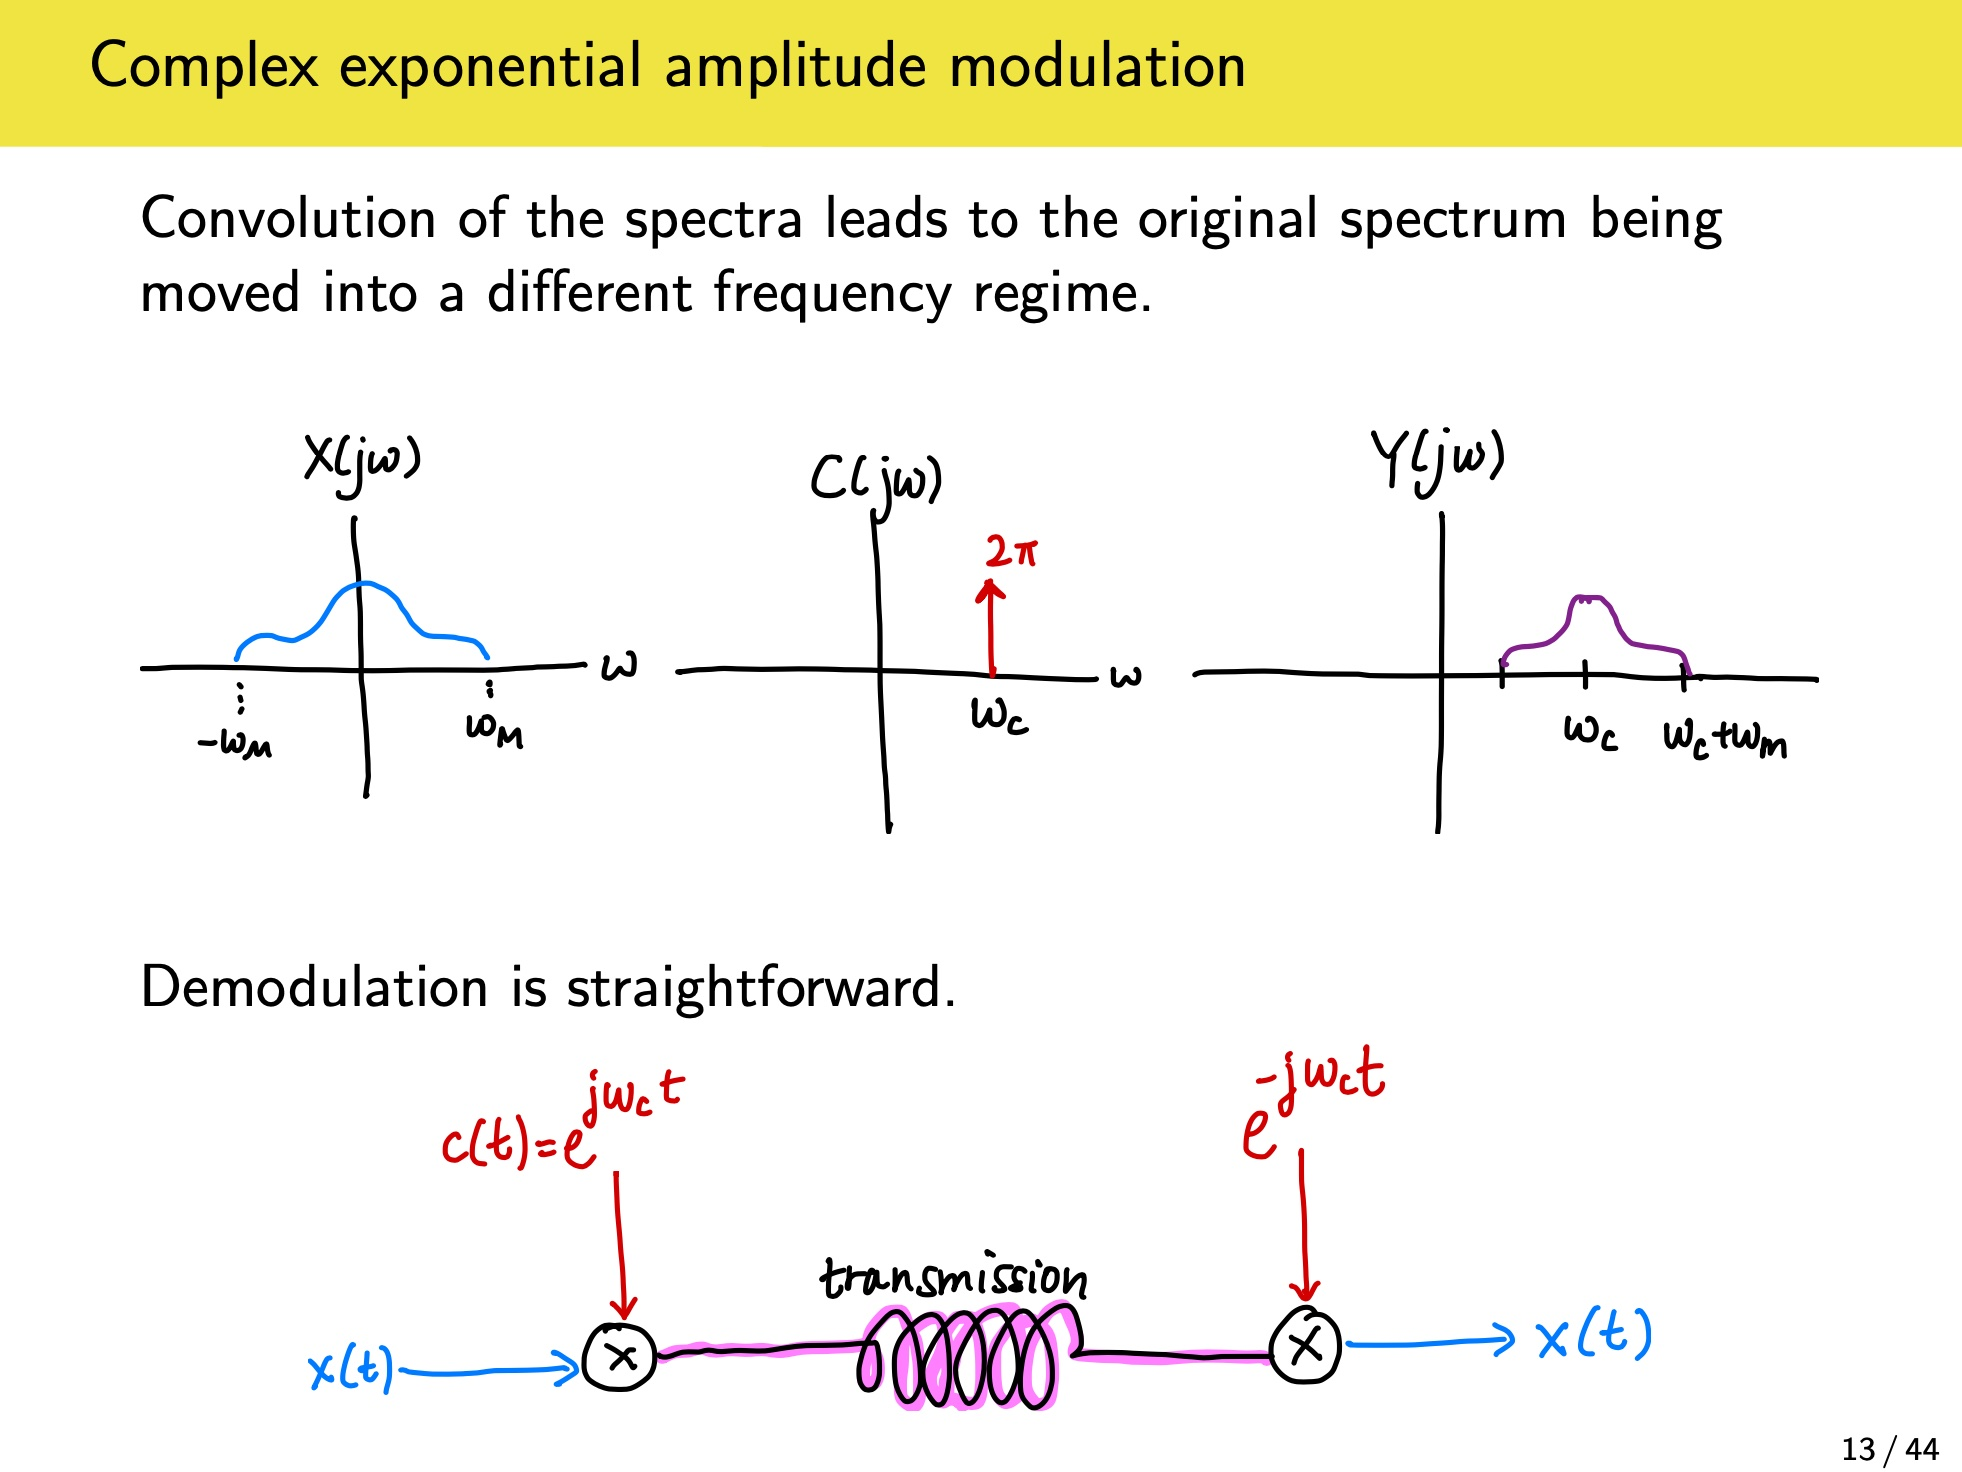
\includegraphics[scale=0.13]{exponential-modulation.jpg}
\pagebreak


\sheader{Amplitude Modulation using Sinusoids} When using sinusoids, there exist some 
more uances. Since the frequency spectrum of a sinusoid has both a positive and 
a negative part, then two signals are outputs of the convolution of the carrier signal 
and the original signal. It also is more challenging since a the frequency spectrum of a 
sinusoid is also scaled down by $\frac{1}{2}$. Hence, when demodulating the signal,
we require that it is subsequently band-pass filtered and applied a gain of 2.

\begin{enumerate}
    \item Original signal $x(t)$ is multiplied by the carrier signal $c(t) = \cos(\omega_c t)$ $y(t) = x(t)c(t)$.
    \item Frequency spectrum of the broadcast $y(t)$ has two parts, one centered at $\omega_c$ and $-\omega_c$. 
    Both parts have amplitude of $A/2$, where $A$ was the original amplitude of $x(t)$.
    \item Modulated signal is broadcasted/transmitted.
    \item Modulated signal is demodulated with a signal $c'(t) = \cos(\omega_c t)$, which
    produces a signal with frequency bands centered at $-2\omega_c$, $0$, and $2\omega_c$.
    Bands centered at $\pm 2\omega_c$ have amplitude $A/4$, whereas the frequency band 
    centered at $0$ has amplitude $A/2$.
    \item To elimate the unwanted bands and return the signal to the correct amplitude, 
    the frequencies are low passed with a cutoff frequency of $\omega_C$, and 
    applied a gain of 2.
\end{enumerate}

For calculations involving sinusoidal amplitude modulations, sine and cosine functions are
often multiplied together. Hence, it is important to remember some key trigonemetric identities:
\begin{align*}
    \sin\theta\cos\theta = \frac{1}{2}\sin(2 \theta) && \cos^2\theta = \frac{1}{2}\left( 1 + \cos(2 \theta)\right)\\
    && \sin^2\theta = \frac{1}{2}\left(1 - \cos(2\theta)\right) 
\end{align*}

\header{Asynchronous Demodulation}
For all of the instances above, we assumed that there was no phase shift in the signal $\theta_c = 0$.
Hence, since phase cannot always be synchronized, we must consider the case in which 
there exists some phase shift. An analysis of asynchronous demodulation is as follows,
for a carrier signal $c(t)$ with phase shift $\theta_c$, and a demudlating signal $c'(t)$
with a phase shift of $\phi_c$.
\begin{align*}
    w(t) &= \cos(\omega_c t + \theta_c)\cos(\omega_c t + \phi_c)x(t)\\
    &= \left[\frac{1}{2} \cos (\theta_c - \phi_c) + \frac{1}{2} \cos \left(2 \omega_c t + \omega_c + \phi_c\right)\right] x(t)\\
    &\textrm{(after application of the low pass filter)}\\
    x_r(t) &= \frac{1}{2}\cos(\theta_c - \phi_c)x(t)
\end{align*}
Since this yields undesireable effects throughout a system to deal with inconsistent gains,
which could decrease signal fidelity, we introduce the idea of amplitude modulation, which 
involves sending a copy of the carrier signal alongside the original signal. Given some assumptions:
\begin{itemize}
    \item $x(t)$ is always positive
    \item $\omega_c$ is much larger than $\omega_m$,
\end{itemize}
an ``envelope detector'' can be constructed, which has the effect of detecting the carrier 
signal sent along with the modulated signal, so that the modulated signal can be 
effectively demodulated using the original carrier signal. This synchronizes the 
modulation and demodulation processes so no signal is lost.
\gap
\sheader{Modulation Index} For a transmission signal of the form $(A + x(t))\cos(\omega_c t)$.
Then the \textit{modulation index} is defined as:
\begin{align*}
    m = \frac{K}{A}
\end{align*}
Where $K$ is the maximal amplitude of $x(t)$ such that $|x(t)| \leq K$. 

\pagebreak

\header{Frequency Division Multiplexing}
A common implementation of modulation is the concept of \underline{frequency division multiplexing}.
Frequency division multiplexing is where band limited signals are modulated to different 
frequencies, such that they can all occupy different, distinct, and non-overlapping regions 
of a frequency spectrum of a single signal. Hence, thre needs to be some way of 
extracting certain signals out of the composite signal. For this there are generally two 
phases:
\begin{enumerate}
    \item A bandpass filter before demodulation.
    \item A low pass filter after demodulation.
\end{enumerate}

\header{Single-Sideband Modulation}
When sending multiple signals on one signal, modulation by a sinusoid results in the 
transmission of both positive and negative frequencies, and hence a waste in energy required 
to send both frequencies. Hence, we introduce the concept of single-sideband modulation.
In single sideband modulation, we eliminate half of the frequencies of a given signal, such that
only one half of the band is actually transmitted. The mechanism for how this happens can
be observed:

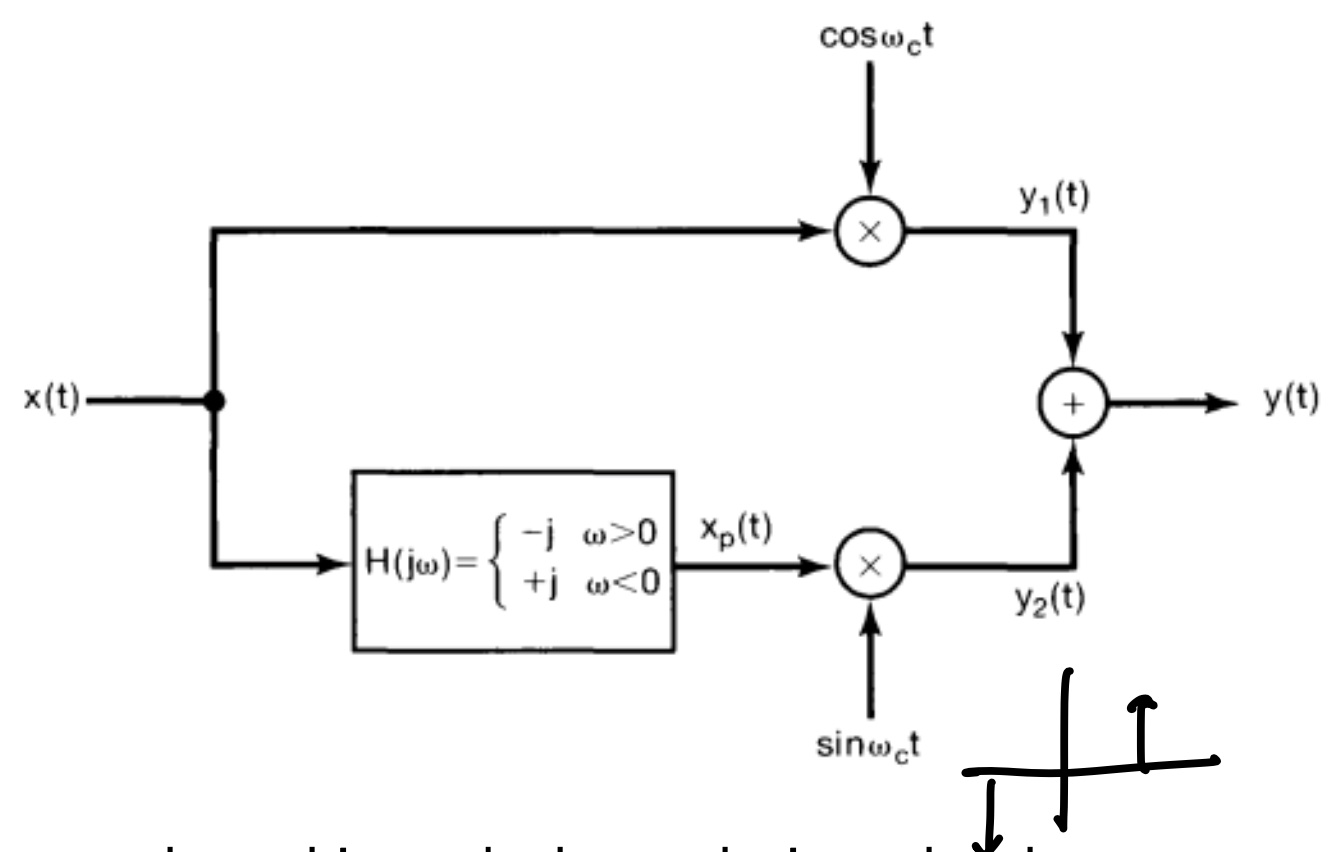
\includegraphics[scale=0.2]{single-sideband.jpg}
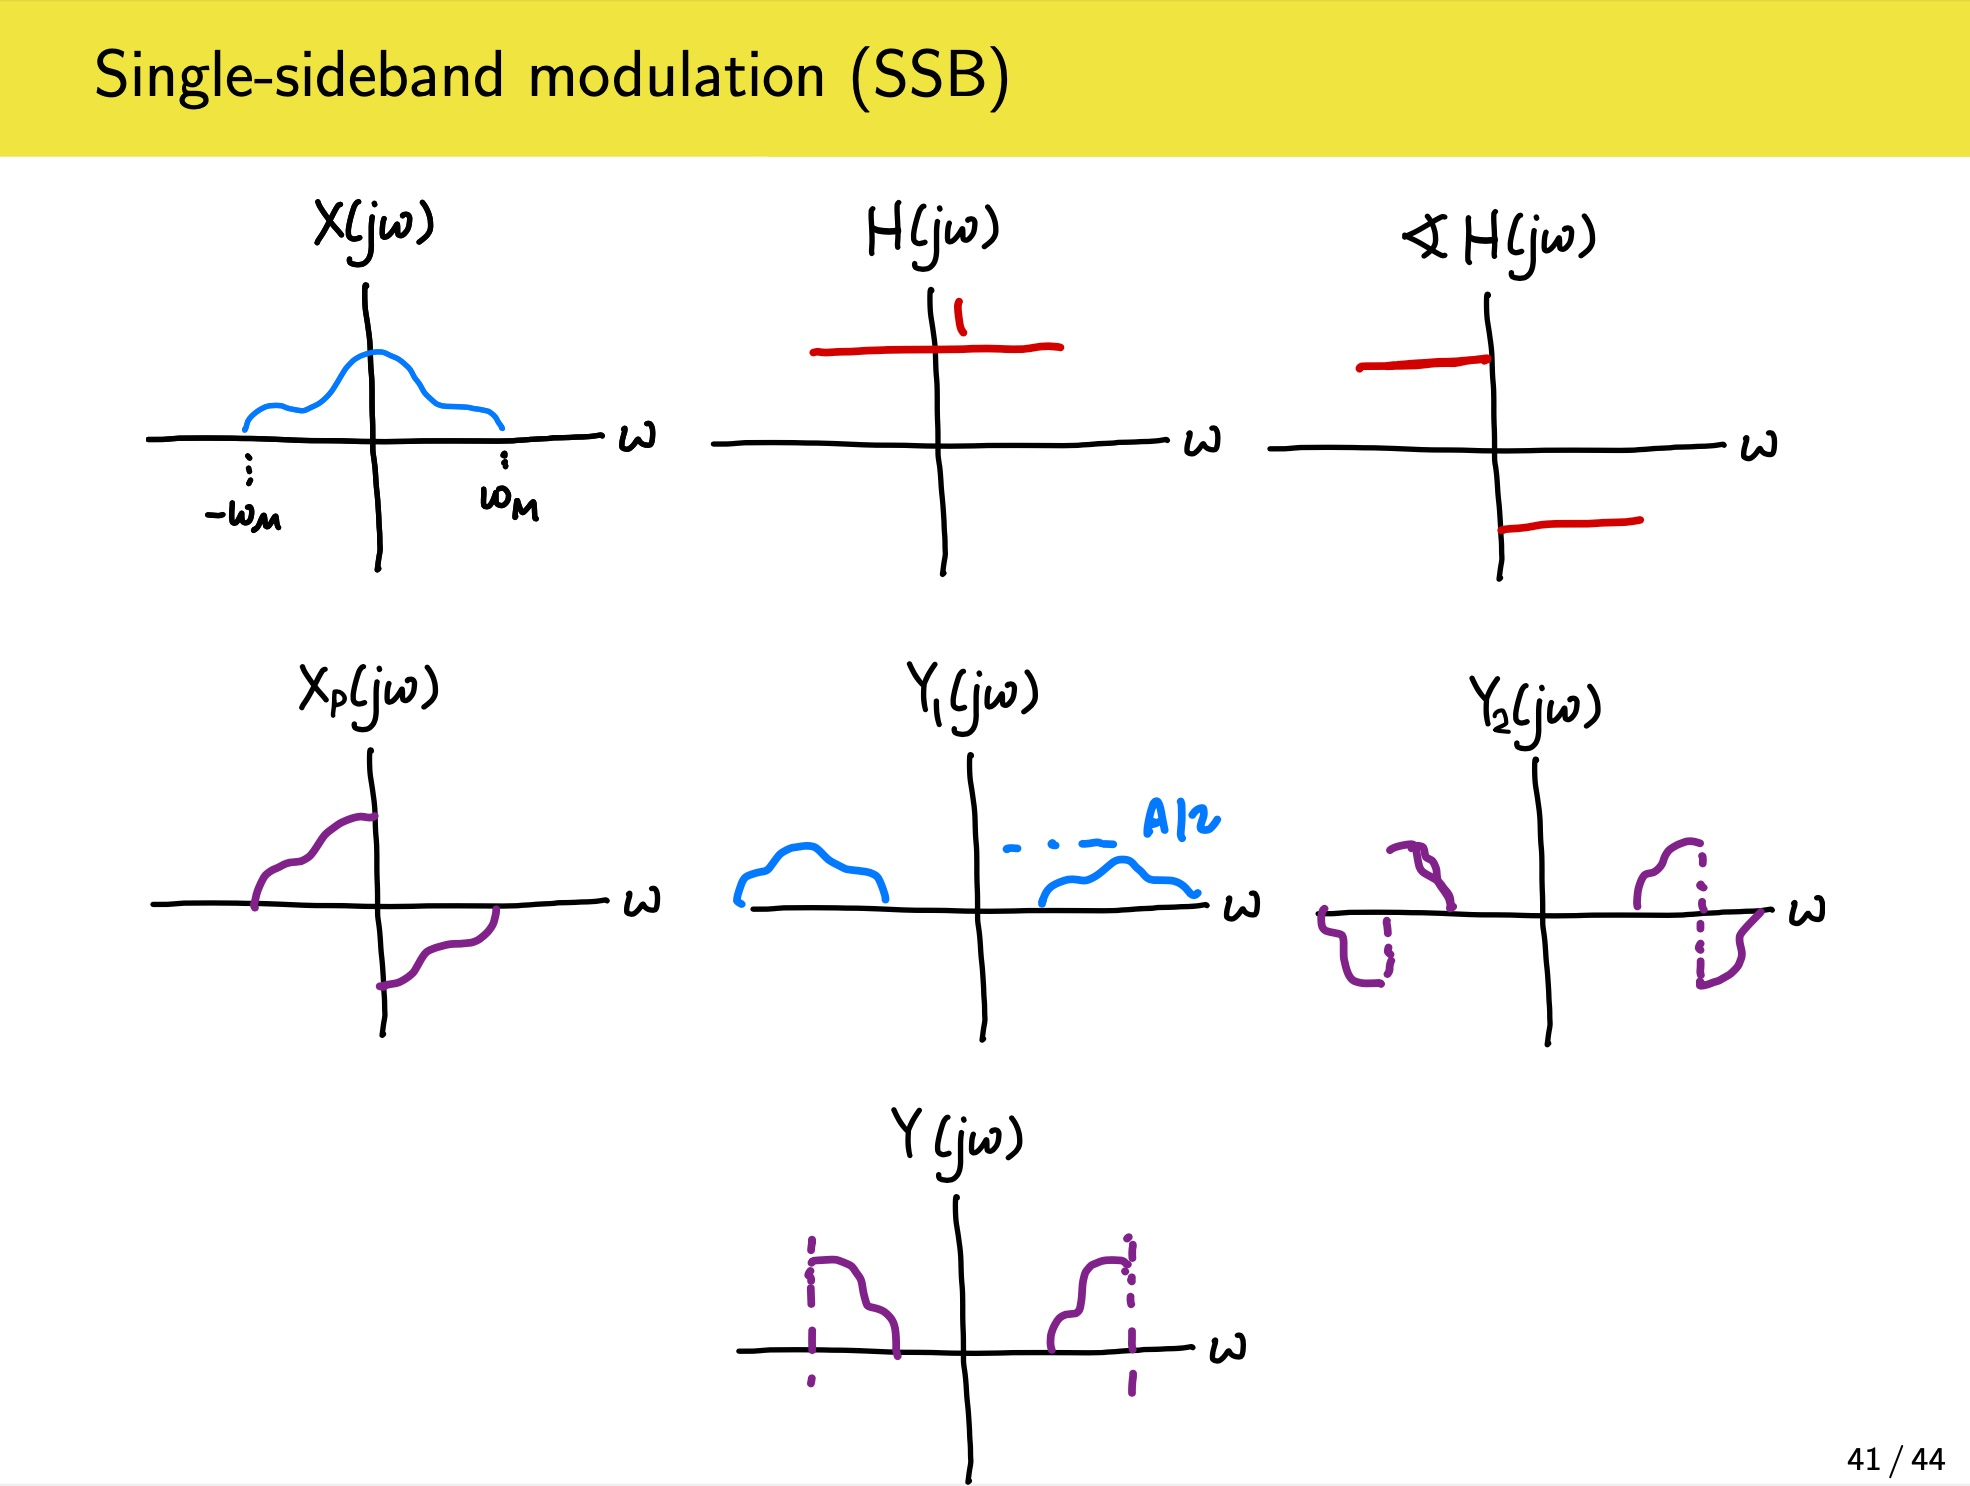
\includegraphics[scale=0.1]{single-sideband-2.jpg}

\header{Discrete Time Sinusoidal Amplitude Modulation}
There exist some important differences when modulating in discrete time. The first is that 
due to everything being in discrete time, one must be cognisant of frequency replication and 
aliasing. It is also important to note what a cosine wave looks like in the frequency 
domain:

\begin{center}
    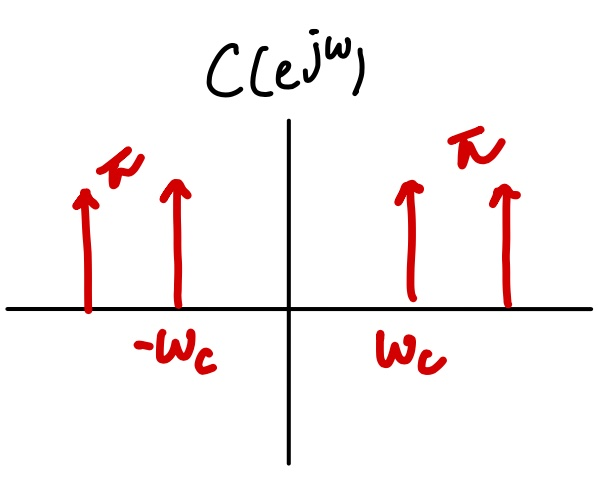
\includegraphics[scale=0.2]{cosine-dt.jpg}
\end{center}

Thus, we are required to impose some conditions on $\omega_c$ and $\omega_n$:
\begin{itemize}
    \item $\omega_c > \omega_n$
    \item $\omega_c < \pi - \omega_n$
\end{itemize}
without these conditions, the signal will suffer from aliasing effects.

\pagebreak

\header{The Laplace Transform}
As we saw with the Fourier transform, there were places in which the Fourier transform 
was not always possible since the integral defining the Fourier transform diverged. 
Hence, we can introduce the \underline{Laplace Transform}, which outlines a more general 
case of the Fourier transform, adding a real constant instead of the purely imaginary 
$\jomega$ which defined the Fourier transform. With this additional real term $\sigma$,
more signals/functions can be transformable, however, there are additional conditions 
which arise, which will be explored while discussing regions of convergence. Hence,
we can define the Laplace transform as:
\begin{align*}
    X(s) = \Laplace\curly{x(t)}  \equiv \int_{-\infty}^\infty e^{-st}x(t)dt
\end{align*}
Where $s = \sigma + \jomega$.
\gap
Since the Fourier and Laplace transforms differ by only the $\sigma$ term in the 
complex exponential, we can take out the complex exponential, and write the Laplace
transform in terms of the the Fourier transform.
\begin{align*}
    \Laplace\curly{x(t)} = \Fourier\curly{e^{-\sigma t} x(t)}
\end{align*}
\sheader{Regions of Convergence} Due to the ``adjustment factor'' that $\sigma$ is, it allows the Laplace transform to 
exist in some regions, where a Fourier transform does not. Hence, we introduce the concept 
of a \underline{region of convergence} of a function, that describes where a function's 
Laplace transform may exist. However, it is important to note that functions may have the 
same algebraeic Laplace transform, but differing regions of convergence. 
\gap
It is also important to note that if a function is a sum of functions, then the region 
of convergence is the region of convergence that allows all of the functions' Laplace 
transforms to exist.
\gap
\sheader{Pole-Zero Plots} Oftentimes, the Laplace transform results in rational 
polynomials of $s$. Generally, under factorization, the roorts of these polynomials are 
shown on a \underline{pole-zero plot}. In such plots:
\begin{itemize}
    \item Numerator factors are called \textbf{zeroes} and symbolized as $\circ$ on plots.
    \item Denominator factors are called \textbf{poles} and symbolized as $\times$ on plots.
\end{itemize}
The region of convergence also has some nice properties:
\begin{itemize}
    \item If the region of convergence does not contain the $\jomega$ axis, then the 
    Fourier tranform does not converge.
    \item The region of convergence of a rational Laplace transform contains no poles.
\end{itemize}
We can also extrapolate signal attributes from various patterns on a region of convergence plot
(pole-zero plot):
\begin{itemize}
    \item \sheader{Finite Length Signals} The reigon of convergence plot spans the 
    entire real axis.
    \item \sheader{Left Sided Signals} For signals that only exist on the left side of 
    some boundary (they are infinite in the negative direction), then the region of 
    convergence exists only to the left of some value $s < \sigma_L$.
    \item \sheader{Right Sided Signals} For signals that only exist on the right side 
    of some boundary (they are infinite in the positive direction), then the region of
    convergence exists only to the right of some value $s > \sigma_R$.
    \item \sheader{Infinite Signals} For signals with no bounds, there \textit{may} exist 
    a region of convergence between some $\sigma_L < s < \sigma_R$.
\end{itemize}
Since these are all biconditionals, then the converse is also true.
\gap
Since a region of convergence can never contain a pole, then for each region between 
poles, there is a possible region of convergence for a given signal, and thus a 
different time domain signal that could represent a Laplace transform.

\pagebreak

\sheader{Properties of the Laplace Transform}\\
\begin{tabular}{| l | c | c | c|}
\hline
Property & Unmodified Transform & Modified Transform & ROC \\
\hline 
Linearity & $\displaystyle x_1(t) \Laplacearrow X_1(s)$ \,\,\, $\displaystyle x_2(t) \Laplacearrow X_2(s)$ & $\displaystyle ax_1(t) + bx_2(t) \xleftrightarrow{\Laplace} aX_1(s) + bX_2(s)$ & contains $R_1 \cap R_2$\\
\hline
Time Shifting & $x(t) \Laplacearrow X(s) $ & $\displaystyle x(t - t_0) \Laplacearrow e^{-st_o}X(s)$ & $R$\\
\hline
$s$ Shifting & $\displaystyle x(t) \Laplacearrow X(s)$ & $\displaystyle e^{s_0 t}x(t) \Laplacearrow X(s- s_0)$ & $R + \textrm{Re}(s_0)$\\
\hline
Time Scaling & $\displaystyle x(t) \Laplacearrow X(s)$ & $\displaystyle x(at) \Laplacearrow \frac{1}{|a|}X\left(\frac{s}{a}\right)$ & $aR$\\
\hline 
Time Reversal & $\displaystyle x(t) \Laplacearrow X(s)$ & $\displaystyle x(-t) \Laplacearrow X(-s)$ & $-R$\\
\hline
Conjugation & $\displaystyle x(t) \Laplacearrow X(s)$ & $\displaystyle x^*(t) \Laplacearrow X^*(s^*)$ & $R$\\
\hline 
Convolution & $\displaystyle x_1(t) \Laplacearrow X_1(s)$ \,\,\, $\displaystyle x_2(t) \Laplacearrow X_2(s)$ & $\displaystyle x_1(t) \ast x_2(t) \Laplacearrow X_1(s)X_2(s)$ & contains $R_1 \cap R_2$\\
\hline
Time Differentiation & $\displaystyle x(t) \Laplacearrow X(s)$ & $\frac{dx(t)}{dt} \Laplacearrow sX(s)$ & contains $R$\\
\hline 
$s$ Differentiation & $\displaystyle x(t) \Laplacearrow X(s)$ & $-tx(t) \Laplacearrow \frac{dx(s)}{ds}$ & $R$\\
\hline
\end{tabular}
\gap
\sheader{Causality} For a signal to be causal, the transfer function $H(s)$
of its impulse resoponse $h(t)$ has to be right sided. That is, the ROC is the right-half 
plane to the right of the right-most pole.
\gap
\sheader{Stability} For a signal to be stable, the transfer function $H(s)$ 
must contain the entire $\jomega$ axis $\textrm{Re}(s) = 0$, \textbf{and} there are 
not more zeros than poles.
\gap
\sheader{Differential Equations} The same principle for differential equations holds in 
the Laplace domain as the Fourier domain:
\begin{align*}
    H(s) = \frac{Y(s)}{X(s)} = \frac{\sum_k{x \textrm{ coeffs} \cdot s^k} }{\sum_k{y \textrm{ coeffs} \cdot s^k}}
\end{align*}

\header{Applications of Laplace Transforms}
An important application of Laplace tranforms are in the implmentation of Feedback systems.
A feedback system takes the following form:
\begin{center}
    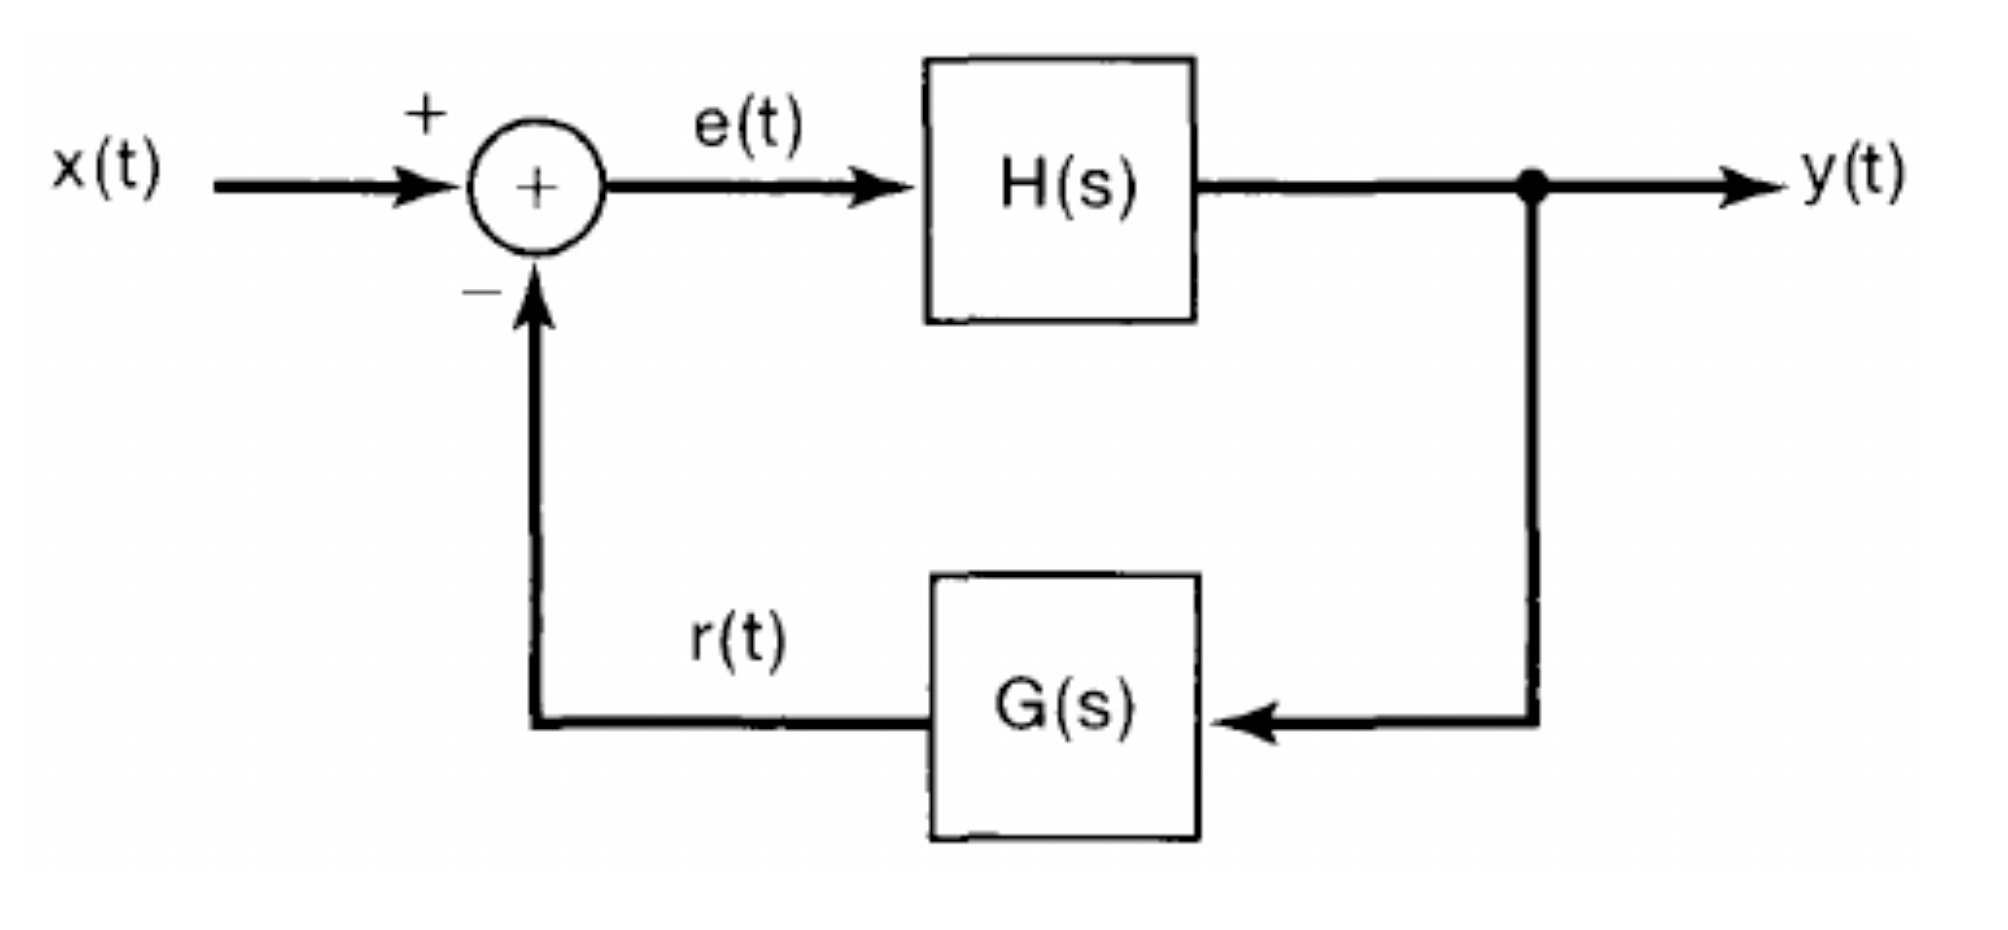
\includegraphics[scale=0.15]{feedback-system.jpg}
\end{center}
Hence, through some algebra, we cand define the transfer function for the overall system
$Q(s)$ to be:
\begin{align*}
    Q(s) = \frac{Y(s)}{X(s)} = \frac{H(s)}{1 + G(s)H(s)}
\end{align*}
Given the form of this transfer function $Q(s)$, we can create systems that solve important 
problems:

\pagebreak

\sheader{Inverse Systems} An inverse system has the ability to reverse a system. They 
are generally laid out in the following form:

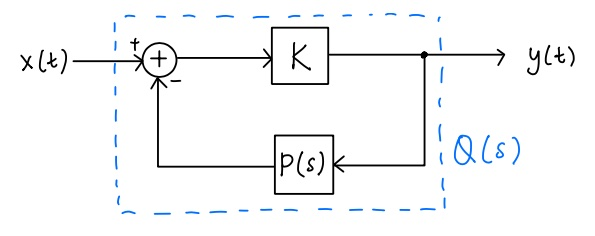
\includegraphics[scale=0.3]{inverse-system.jpg}\\
Where $K$ denotes a gain of $K$. Hence, under analysis of the transfer function $Q(s)$,
we can deduce that:
\begin{align*}
    \lim_{K \gg P(s)} Q(s) = \lim_{K \gg P(s)}{\frac{K}{1 + KP(s)}} \approx \frac{1}{P(s)}.
\end{align*}
Hence, this has the effect of ``inverting the signal''.
\gap
\sheader{Stabilizing Systems} The other system that is useful is a stabilizing system. Given 
some signal with a pole $H(s) = \frac{b}{s-a}$, then it follows that:
\begin{align*}
    Q(s) &= \frac{H(s)}{1 + KH(s)}\\
    &= \frac{b}{(s-a)(1 + K \frac{b}{s-a})}\\
    &= \frac{b}{s - a + Kb}\\
    Q(s) &= \frac{b}{s - (a - Kb)}.
\end{align*}
Hence, if we make $kB > a$, we can move the pole to be on the left side of the $\jomega$ axis,
such that the system is stable.
\gap
\header{Z-Transforms}
Like much of the techniques in this course, there is a discrete time analouge for the 
Laplace transform, called the \underline{Z-transform}. We define the $Z$ transform as:
\begin{align*}
    X(z) = \sum_{n = - \infty}^\infty x[n]z^{-n}.
\end{align*}
Where $z = re^\jomega$. \gap
This can also be put in terms of a discrete-time Fourier transform:
\begin{align*}
    X(re^\jomega) = X(z) = \Fourier\curly{x[n]r^{-n}}.
\end{align*}
\header{Regions of Convergence} However, it is to be said that regions of convergence look
different in Z-transforms as opposed to Laplace transforms. Since $z$ is in the form of 
a complex exponential, the regions of convergence find themselves on a circular domain. 
Hence, the unit circle is the $z$ axis, which is analogous to the $\jomega$ axis in the 
Laplace transform.\\
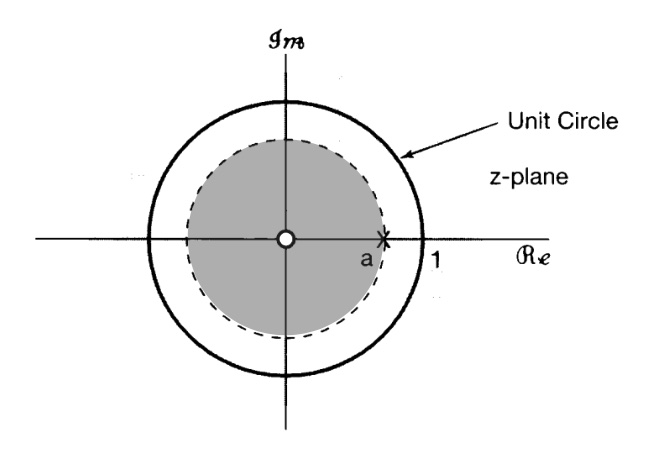
\includegraphics[scale=0.2]{z-roc.jpg}

\pagebreak

Hence, we can define some properties for the regions of convergence of the Z-transform:
\begin{itemize}
    \item The ROC must contain the unit circle for the DTFT to converge.
    \item All ROCs do not contain poles.
    \item All ROCs are rings in the $z$-plane centered around the origin.
\end{itemize}
Patterns of convergence are also similar for the Z-Transform:
\begin{itemize}
    \item If $x[n]$ is of finite duration, then the ROC is the entire $z$-plane,
            except possibly $z = 0$ and $z = \infty$.
    \item If $x[n]$ is a right-sided sequence, and the circle $|z| = r_0$ is in the ROC
            then all finite values of $z$ for which $|z| > r_0$ will also be in the ROC.
    \item if $x[n]$ is a left-sided sequence, and if the circle $|z| = r_0$ is in the ROC,
            then all values of $z$ for which $0 < |z| < r_0$ will also be in the ROC.
    \item if $x[n]$ is two-sided, and if the circle $|z| = r_0$ is in the ROC,
            then the ROC will consist of a ring in the $z$-plane that includes the circle 
            $|z| = r_0$.
\end{itemize}
\begin{center}
    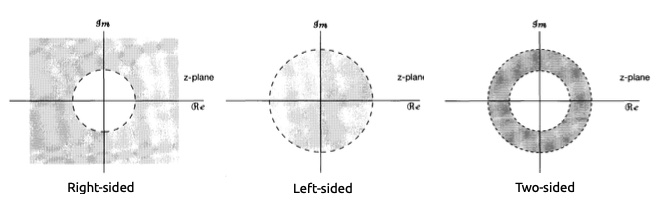
\includegraphics[scale=0.6]{z-roc-cases.jpg}
\end{center}
\sheader{Inverse Z-Transforms} Generally, these are done with a Z-Transform table, but
power series expansions are often a helpful tool, such as for $\log$ functions.
\gap
\sheader{Properties of the Z-Transform}\\
\begin{tabular}{ | l | c | c | }
    \hline
    Property & Form & ROC\\
    \hline
    Linearity & $ax_1[n] + bx_2[n] \zarrow aX_1(z) + bX_2(z)$ & contains $R_1 \cap R_2$\\
    \hline
    Time Shift & $x[n - n_0] \zarrow x^{-n_0}X(z)$ & $R$, may add/delete $0$ or $\infty$\\
    \hline
    Time Reversal & $x[-n] \zarrow X\left(\frac{1}{z}\right)$ & $\frac{1}{R}$\\
    \hline
    Time Expansion (insertion of $k-1$ zeroes) & $X_{(k)}[n] \zarrow X(z^k)$ & $R^{\frac{1}{k}}$\\
    \hline
    $z$ Scaling & $z_0^n x[n] \zarrow X\left(\frac{z}{z_0}\right) $ & $|z_0|\cdot R$\\
    \hline
    Conjugation & $x^*[n] \zarrow X^*(z^*)$ & $R$\\
    \hline
\end{tabular}
\gap
\sheader{Z-Transform and Causality} A Discrete Time LTI system with a rational Z-Transform 
is causal if:
\begin{itemize}
    \item The ROC is the exterior of circle outside the outermost pole.
    \item The order of the numerator in the transfer function $H(z)$ does not exceed the denominator.
\end{itemize}
\sheader{Z-Transform and Stability} A Discrete Time LTI system is stable if:
\begin{itemize}
    \item The ROC includes the unit circle $|z| = 1$.
\end{itemize}
\sheader{Difference Equations}
Similar to everything else:
\begin{align*}
    \sum_{k = 0}^N a_k y[n-k] &= \sum_{k = 0}^M b_k x[n -k]\\
    H(z) = \frac{Y(z)}{X(z)} &= \frac{\sum_k x \textrm{ coeffs} \cdot z^{-k}}{\sum_k y \textrm{ coeffs} \cdot z^{-k}}
\end{align*}
Remeber: the sign of $k$ is important.
\gap
\header{Feedback Systems with Z-Tranforms}
Very similarly to Laplace transforms, we can have feedback systems in Z-Transforms. 
They generally take the following form:\\
\begin{center}
    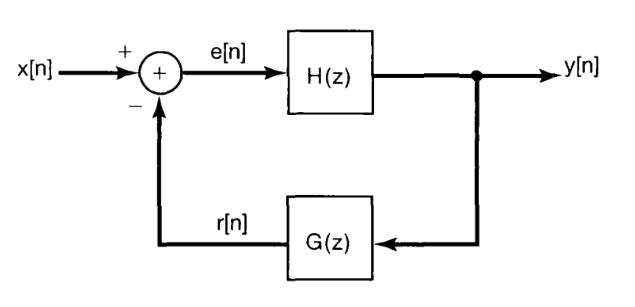
\includegraphics[scale=0.35]{z-feedback.jpg}
\end{center}
Hence, the transfer function takes the same form:
\begin{align*}
    Q(z) = \frac{Y(z)}{X(z)} = \frac{H(z)}{1 + G(z)H(z)}.
\end{align*}




\end{document}